\documentclass{article}

% Language setting
% Replace `english' with e.g. `spanish' to change the document language
\usepackage[english]{babel}
% Set page size and margins
% Replace `letterpaper' with `a4paper' for UK/EU standard size
\usepackage[letterpaper,top=2cm,bottom=2cm,left=3cm,right=3cm,marginparwidth=1.75cm]{geometry}
\usepackage{CJKutf8}
% Useful packages
\usepackage{amsmath}
\usepackage{graphicx}
\usepackage{siunitx}
\usepackage[colorlinks=true, allcolors=blue]{hyperref}

\title{Chapter 2: Polynomial Interpolation}
\author{倪爽爽 3210101597\thanks{Email: 3210101597@zju.edu.cn}}


\begin{document}
\begin{CJK}{UTF8}{gbsn}
\maketitle

%\begin{abstract}
%Your abstract.
%\end{abstract}

\section*{A.}

\textbf{Answer: }
Construct function to calculate divided differences
\begin{verbatim}
std::vector<double> dividedDifferences(const std::vector<double>& x, const std::vector<double>& y) {
    int n = x.size();
    std::vector<double> coeffs = y; // Start with y values
    for (int j = 1; j < n; ++j) {
        for (int i = n - 1; i >= j; --i) {
            coeffs[i] = (coeffs[i] - coeffs[i - 1]) / (x[i] - x[i - j]);
        }
    }
    return coeffs;
}
\end{verbatim}
In this function, the size of vector $x$ need to be same as that of vector $y$.\par
Then, we construct function to calculate the Newton interpolation by accumulating.
\begin{verbatim}
    double newtonInterpolation(double x, const std::vector<double>& x_points, const std::vector<double>& coeffs) {
    double result = coeffs[0];
    double product = 1.0;
    for (int i = 1; i < coeffs.size(); ++i) {
        product *= (x - x_points[i - 1]);
        result += coeffs[i] * product;
    }
    return result;
}
\end{verbatim}



\section*{B.}


\textbf{Answer}: 
Construct the function we need:
\begin{verbatim}
    double f(double x) {
    return 1.0 / (1 + x * x);
}
\end{verbatim}
The different divisions can be realized by the function below:
\begin{verbatim}
 for (int n : n_values) {
        // Generate x_i points
        std::vector<double> x_i, y_i;
        for (int i = 0; i <= n; ++i) {
            double x_val = x_min + i * (x_max - x_min) / n;
            x_i.push_back(x_val);
            y_i.push_back(f(x_val));
        }
\end{verbatim}
Using the functions constructed above, we can implement Newton interpolate. 

\begin{verbatim}
    std::cout << "n = " << n << ":\n";
        for (int i = 0; i <= num_points; ++i) {
            double x = x_min + i * (x_max - x_min) / num_points;
            double y_exact = f(x);
            double y_interp = newtonInterpolation(x, x_i, coeffs);
            std::cout << std::fixed << std::setprecision(5) 
                      << "x: " << x << " Exact: " << y_exact << " Interpolated: " << y_interp << "\n";
        }
        std::cout << "\n";
\end{verbatim}
To visualize the result, in the real code we change the output into a $txt$ file. The figure output lies below,
\begin{figure}[h!]
    \centering
    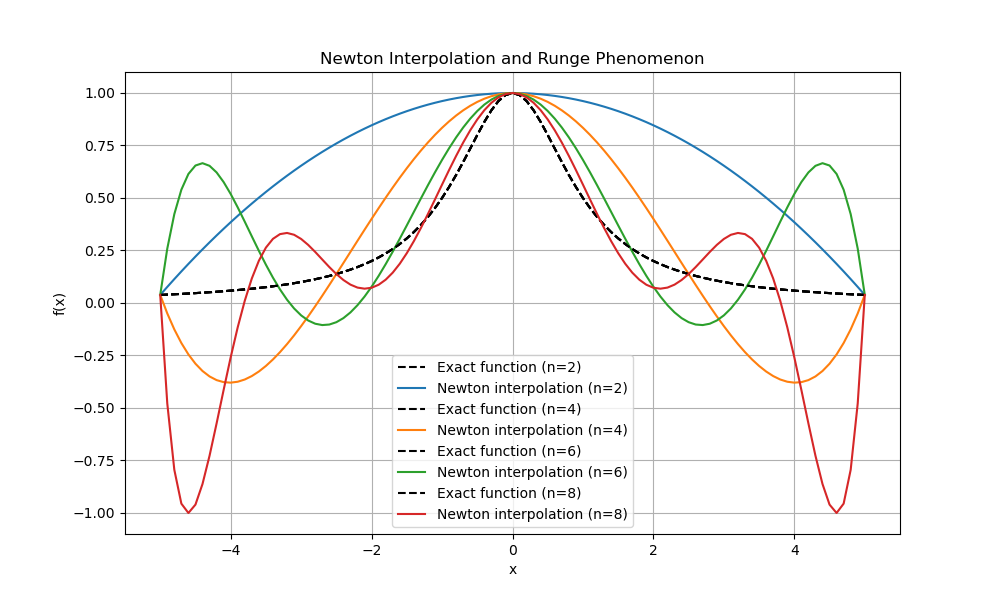
\includegraphics[width=1\linewidth]{Figure_1.png}
\end{figure}

\section*{C.}
\textbf{Answer: }\\
Construct function to calculate Chebyshev nodes for interpolation
\begin{verbatim}
std::vector<double> chebyshevNodes(int n) {
    std::vector<double> nodes;
    for (int k = 0; k < n; ++k) {
        double node = cos(M_PI * (2 * k + 1) / (2 * n));
        nodes.push_back(node);
    }
    return nodes;
}
\end{verbatim}
Similar to the problem B, the output can be showed as below:
\begin{figure}[h!]
    \centering
    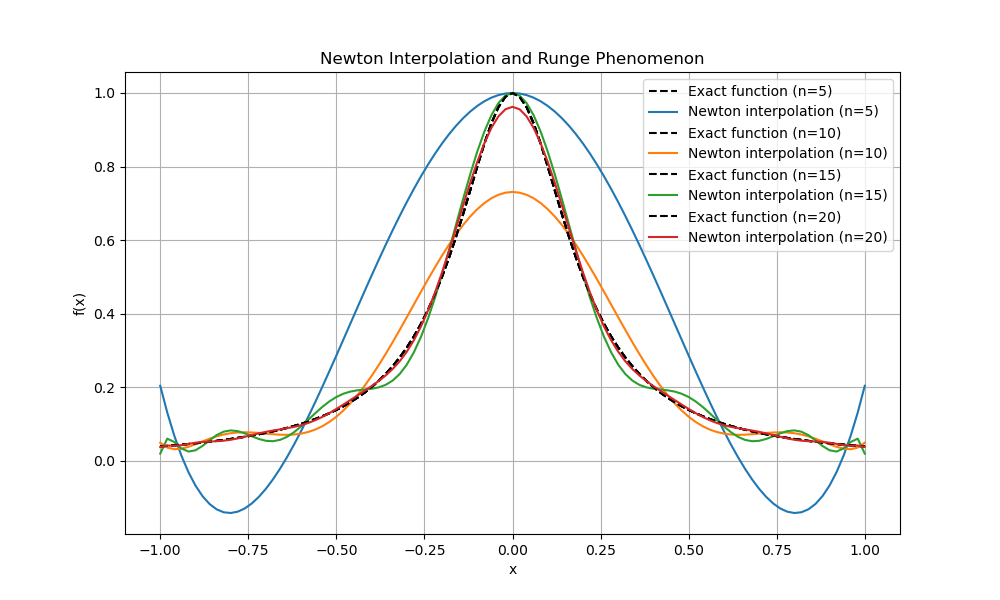
\includegraphics[width=1\linewidth]{Figure_2.png}
    \label{fig:enter-label}
\end{figure}
We can easily see that the accuracy is significantly improved when n increasing.


\section*{D.}

\textbf{Answer: }
The divided difference can be calculated by
$$
dividedDifferences[i] = \frac{
                    dividedDifferences[i] - dividedDifferences[i - 1]} { timePoints[i] - timePoints[i - j]}

$$


If the division is 0, the divided difference can be calculated by
$$
dividedDifferences[i] = velocities[i / 2]
$$


The interpolation can be solved through using the Newton accumulation method.\par
While the result turns out wrong as below,
\begin{verbatim}
Predicted position at t = 10: -977.897 feet
Predicted speed at t = 10: 6.75285e+08 feet/sec
Did the car exceed 81 feet/sec? Yes
\end{verbatim}


\section*{E.}

\textbf{Answer: }
Using the interpolation code mentioned at problem A, we can implement Newton interpolation.
\begin{verbatim}
Predicted weight for Sp1 at day 43: 14640.3 grams
Predicted weight for Sp2 at day 43: 2981.48 grams
Sp1 larvae might survive after another 15 days.
Sp2 larvae might survive after another 15 days.
\end{verbatim}
But the prediction result deviate greatly from the original numbers.  

\section*{F.}
The result can be showed as below
\begin{figure}[h!]
    \centering
    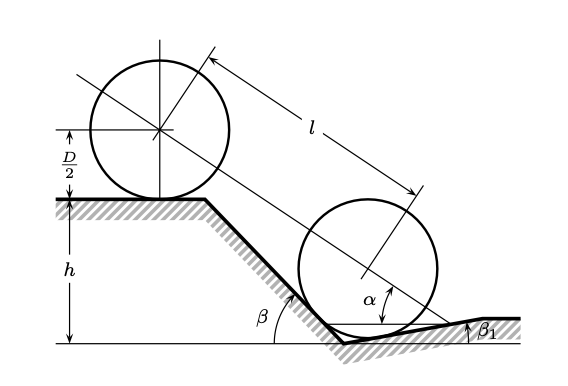
\includegraphics[width=1\linewidth]{F.png}
    \caption{Problem F}
\end{figure}


\section*{Acknowledgments}
During the preparation of this work the author used ChatGPT to solve the questions and polish the language.
In these work, GPT helped me a lot in transferring algorithms to codes and visualization.

%\bibliographystyle{alpha}
%\bibliography{sample}

\end{CJK}
\end{document}